%%%%%%%%%%%%%%%%%%%%%%%%%%%%%%%%%%%%%%%%%%%%%%%%%%%%%%%%%%%%%%%%%%%%%%
% amspaper.tex --  LaTeX2e-based template for submissions to American 
% Meteorological Society Journals, including
%
% JAS 	-- Journal of the Atmospheric Sciences
% JAMC 	-- Journal of Applied Meteorology and Climatology
% JPO 	-- Journal of Physical Oceanography
% MWR 	-- Monthly Weather Review
% JTECH -- Journal of Atmospheric and Oceanic Technology
% WAF 	-- Weather and Forecasting
% JCLI 	-- Journal of Climate
% JHM 	-- Journal of Hydrometeorology
% JAM 	-- Journal of Applied Meteorology
%
% Template developed by B. Papa and S. Cooley, AMS. 
% Email questions to latex@ametsoc.org.
%
% August 12, 2008 (SRC)
%	- Clarified/added header notes, comments throughout
%	- Improved title page
%	- Edited text of document for clarity
%	- Altered list styles to adhere to AMS style, added comments
%	- Removed incorrect commands (i.e., \catcode) (corrects umlaut bug)
%	- Moved non-template commands to ametsoc.sty
%
% August, 2008 - B. Papa
% - Updated to handle two column journal page output
% - Updated text with new/modified instructions
%
%%%%%%%%%%%%%%%%%%%%%%%%%%%%%%%%%%%%%%%%%%%%%%%%%%%%%%%%%%%%%%%%     
%%%%%%%%%%%%%%%%%%%%%%%%%%%%%%%%%%%%%%%%%%%%%%%%%%%%%%%%%%%%%%%%
%																															 %
%				USE THIS TEMPLATE, AMETSOC.STY, AND AMETSOC.BST				 %
%			        OR YOUR TEX FILES WILL NOT BE USED				  		 %
%																															 % 
%%%%%%%%%%%%%%%%%%%%%%%%%%%%%%%%%%%%%%%%%%%%%%%%%%%%%%%%%%%%%%%%
%%%%%%%%%%%%%%%%%%%%%%%%%%%%%%%%%%%%%%%%%%%%%%%%%%%%%%%%%%%%%%%%

%%%%%%%%%%%%%%%%%%%%%%%%%%%%%%%%%%%%%%%%%%%%%%%%%%%%%%%%%%%%%%%%%%%%%
% PREAMBLE
%%%%%%%%%%%%%%%%%%%%%%%%%%%%%%%%%%%%%%%%%%%%%%%%%%%%%%%%%%%%%%%%%%%%%
%
% The following two commands will generate a PDF that follows all the requirements for submission
% and peer review.  Uncomment these commands to generate this output (and comment out the two lines below.)
%
% DOUBLE SPACE VERSION FOR SUBMISSION TO THE AMS
\documentclass[12pt]{article}
\usepackage{ametsoc}
\linenumbers
%
% The following two commands will generate a single space, double column paper that closely
% matches an AMS journal page.  Uncomment these commands to generate this output (and comment
% out the two lines above. FOR AUTHOR USE ONLY. PAPERS SUBMITTED IN THIS FORMAT WILL BE RETURNED
% TO THE AUTHOR for submission with the correct formatting.
%
% TWO COLUMN JOURNAL PAGE LAYOUT FOR AUTHOR USE ONLY
%\documentclass[10pt]{article}
%\usepackage{ametsoc2col}
\usepackage{subfigure}
\usepackage{comment}
\usepackage{verbatim}
\usepackage{fancyvrb}

%
%%%%%%%%%%%%%%%%%%%%%%%%%%%%%%%%%%%%%%%%%%%%%%%%%%%%%%%%%%%%%%%%%%%%%
% ABSTRACT
%
% Enter your Abstract here
%%%%%%%%%%%%%%%%%%%%%%%%%%%%%%%%%%%%%%%%%%%%%%%%%%%%%%%%%%%%%%%%%%%%%
\newcommand{\myabstract}{Tangent linear and adjoint models have been re-developed for the Weather Research and Forecasting (WRF) Model with its Advanced Research WRF dynamic core (WRFPLUS). The automatic differentiation engine (TAPENADE) has been used in the development. The WRFPLUS has the following improvements: 
\begin{itemize}
\item A complete check interface ensures developers to write the tangent linear and adjoint codes in accuracy.
\item To parallelize the WRFPLUS model, we adopted an innovative technique based on the nature duality that existed between MPI communication routines. The Registry in WRF is extended to automatically generate the tangent linear and adjoint of the required communication operations. This approach dramatically speeds up the software development cycle of the parallel tangent linear and adjoint codes and leads to impressive parallel efficiency. 
\item Module interfaces have been constructed for coupling tangent linear and adjoint codes of the WRF with other applications, such as four-dimensional variational data assimilation, forecast sensitivity to observation etc.
\end{itemize}
 }
%
\begin{document}
%
%%%%%%%%%%%%%%%%%%%%%%%%%%%%%%%%%%%%%%%%%%%%%%%%%%%%%%%%%%%%%%%%%%%%%
% TITLE
%
% Enter your TITLE here
%%%%%%%%%%%%%%%%%%%%%%%%%%%%%%%%%%%%%%%%%%%%%%%%%%%%%%%%%%%%%%%%%%%%%
\title{\textbf{\large{Development of the Upgraded Tangent Linear and Adjoint of the Weather Research and Forecasting (WRF) Model}}}
%
% Author names, with corresponding author information. 
% [Update and move the \thanks{...} block as appropriate.]
%
\author{\textsc{Xin Zhang}
				\thanks{\textit{Corresponding author address:} 
				Dr. Xin Zhang, NCAR,MMM, P.O. Box 3000, 
				 Boulder, CO 80307. 
				\newline{E-mail: xinzhang@ucar.edu}}\\
\textit{\footnotesize{National Center for Atmospheric Research, Boulder, Colorado 80307, USA}}
\and 
\centerline{\textsc{Xiang-Yu Huang}}\\% Add additional authors, different institution
\centerline{\textit{\footnotesize{National Center for Atmospheric Research, Boulder, Colorado 80307, USA}}}
\and
\centerline{\textsc{Ning Pan}}\\% Add additional authors, different institution
\centerline{\textit{\footnotesize{Fujian Meteorological Bureau, Fuzhou, Fujian, China}}}
}
%
% The following block of code will handle the formatting of the title page depending on whether
% we are formatting a double column (dc) author draft or a single column paper for submission.
% AUTHORS SHOULD SKIP OVER THIS... There is nothing to do in this section of code.
\ifthenelse{\boolean{dc}}
{
\twocolumn[
\begin{@twocolumnfalse}
\amstitle

% Start Abstract (Enter your Abstract above.  Do not enter any text here)
\begin{center}
\begin{minipage}{13.0cm}
\begin{abstract}
	\myabstract
	\newline
	\begin{center}
		\rule{38mm}{0.2mm}
	\end{center}
\end{abstract}
\end{minipage}
\end{center}
\end{@twocolumnfalse}
]
}
{
\amstitle
\begin{abstract}
\myabstract
\end{abstract}
\newpage
}
%%%%%%%%%%%%%%%%%%%%%%%%%%%%%%%%%%%%%%%%%%%%%%%%%%%%%%%%%%%%%%%%%%%%%
% MAIN BODY OF PAPER
%%%%%%%%%%%%%%%%%%%%%%%%%%%%%%%%%%%%%%%%%%%%%%%%%%%%%%%%%%%%%%%%%%%%%
%
\section{Introduction}

During the past two decades, the use of the adjoint technique in meteorology and oceanography has been rapidly increasing.  The adjoint model is a powerful tool in many applications, such as data assimilation, parameter estimation, sensitivity analysis etc. (\cite{Errico1992};\cite{Errico1997};\cite{Rabier1996};\cite{Langland1999};\cite{Li1999};\cite{Xiao2002};\cite{Xiao2008};\cite{Kleist2005a};\cite{Kleist2005b})

The Weather Research and Forecasting (WRF) modeling system (\cite{Skamarock2005}) is a multi-agency effort intended to provide a next-generation mesoscale forecast model and data assimilation system to advance both the understanding and prediction of mesoscale weather and accelerate the transfer of research advances into operations. The WRF model is designed to be an efficient massively parallel computing code to take advantage of advanced high-performance computing systems. The code can be configured for both research and operations and offers numerous physics options. WRF is maintained and supported as a community model to facilitate wide use internationally, for research, operations, and teaching. It is suitable for a broad span of applications across scales ranging from large-eddy to global simulations. Such applications include real-time NWP, data assimilation development and studies, parameterized-physics research, regional climate simulations, air quality modeling, atmosphere-ocean coupling, and idealized simulations. As of this writing, the number of registered WRF users exceeds 19905, and WRF is in operational and research use around the world.

The first version of adiabatic WRF tangent linear (TLM) and adjoint model (ADM) system (WAMS) was developed by NCAR around 2007 (\cite{Xiao2008}). It has been used in the adjoint sensitivity analysis (\cite{Xiao2008}) and four-dimensional variational data assimilation (4D-Var) (\cite{Huang2009}). In the past few years, due to the hand-coded parallellisation, WAMS has failed to follow the rapid development of WRF model and data assimilation system (WRFDA)(\cite{Barker2012}). The growing gap between WAMS and WRF/WRFDA makes WAMS inconvenient to be used with other systems. Furthermore, because WAMS uses the disk input/output (I/O) for storing basic states and exchanging data, parallel efficiency is unsatisfactory on modern high performance computers with distributed memory parallelization, especially, for 4D-Var applications.  
 
Encouraged by the rapid developments of  4D-Var, cloud analysis, forecast sensitivity to observations and chemistry data assimilation, we re-developed the WRF tangent linear model and adjoint model (called WRFPLUS) based on the latest repository WRF. Compared with the WAMS developed by \cite{Xiao2008} and \cite{Huang2009}, the new system is an all-in-one system which includes the WRF full-physics forward model (FWM), tangent linear model (TLM) and adjoint model (ADM); it also includes the tangent linear check and adjoint check procedure. A set of module interfaces is developed for easily coupling WRFPLUS with other systems such as data assimilation and adjoint sensitivity applications.  An innovative approach has been applied to develop the parallel code which dramatically reduces the software development cycle of parallel TLM and ADM, and the derived parallel TLM and ADM have better parallel efficiency compared to the FWM.

The purpose of this paper is to describe the technical aspects of the newly developed WRFPLUS model. A brief introduction of the development of WRFPLUS is presented in section 2, followed by demonstration of the linearity and adjoint tests in section 3. A detailed description of parallelization strategy for the tangent linear and adjoint codes, as well as the parallel performance are in section 4. Section 5 introduces the module interfaces which are constructed in WRFPLUS for coupling purposes, such as in WRF 4D-Var. The concluding remarks are given in section 6.

\section{Description of the WRF tangent linear and adjoint model}

After the release of WRF model version 3.2, we started to use TAPENADE (\cite{Hascoet2004T2u}) to re-develop the tangent linear and adjoint models of the WRF ARW core based on the latest WRF model. The development of WRFPLUS system follows the same three phases proposed by \cite{Xiao2008}. Firstly, numerical experiments were conducted to make sure the adiabatic version of WRF with simplified physics paramterisation routines can produce the major features that the full-physics model does. Secondly, the tangent linear model and its adjoint were generated by TAPENADE and modified manually whenever necessary. The third step is to verify the correctness of the tangent linear and adjoint models.

TAPENADE is a source-to-source automatic differentiation (AD) tool for programs written in Fortran 77-95, i.e. TAPENADE generates a TLM or ADM from the source code of a given model. Like other AD tools, TAPENADE has difficulty to handle some of the complicate codes in WRF, such as third-order Runge-Kutta large time steps and small acoustic time steps (\cite{Xiao2008}), and manual intervention is necessary to check and improve the TAPENADE generated code. To represent first-order physical effects on the model evolution while also minimizing the code length to make developing its adjoint simple, and to allow the code to run quickly in the iterations required to minimize the cost function, we adopted three simplified physics packages which have maximum impact on the forecast compared to a no-physics model. They are surface friction, cumulus parameterization and large-scale condensation developed by Jimy Dudhia (personal communication), which are similar to the those physics packages in WAMS (\cite{Xiao2008}).

\section{Linearity test and adjoint test}

It is important and necessary to test the TLM consistency with the FWM and the ADM consistency with the TLM before they are used in any real application (\cite{Vukicevic1991}; \cite{Errico1992}; \cite{Gilmour2001}). We developed the tangent linear and adjoint check procedure following \cite{Navon1992}.

Let $\mathbf{f}(\mathbf{x})$, $g\_\mathbf{f}(\mathbf{x},g\_\mathbf{x})$ and $a\_\mathbf{f}(\mathbf{x},a\_\mathbf{x})$ denote a forward, tangent linear and adjoint model, respectively, where $\mathbf{x}$, $g\_\mathbf{x}$ and $a\_\mathbf{x}$ is column vector of model state variables, perturbations of state variables and adjoint of state variables, respectively. The correctness of tangent linear model can be tested as:
\begin{equation}
\label{tlcheckf}
{\Phi(\lambda)}={\frac{\|\mathbf{f}(\mathbf{x}+{\lambda}g\_\mathbf{x})-\mathbf{f}(\mathrm{x})\|}{{\|g\_\mathbf{f}(\mathbf{x},{\lambda}g\_\mathbf{x})\|}}},  \lim_{\lambda \rightarrow 0}{\Phi(\lambda)}=1
\end{equation}
where $\|\|$ denotes the norm of the vector.
The adjoint relation is tested by :
\begin{equation}
\label{adcheck}
\langle g\_\mathbf{f}(\mathbf{x},g\_\mathbf{x}),g\_\mathbf{f}(\mathbf{x},g\_\mathbf{x}) \rangle = \langle a\_\mathbf{f}(\mathbf{x},g\_\mathbf{f}(\mathbf{x},g\_\mathbf{x}),g\_\mathbf{x} \rangle
\end{equation}
If the tangent linear and adjoint codes are correct, the above two relations should hold up to the machine accuracy. Because different model variables have different magnitudes, we also design the capability to perform checks on individual variables separately. We performed the tangent linear and adjoint check with the test case being integrated up to 24h. We sequentially reduced the initial perturbations by a factor ($\lambda$) of $10$ and repeatedly calculate $\Phi(\lambda)$ in Eqs. (\ref{tlcheckf}) on NCAR IBM machine with 64 bits precision. Table \ref{tlcheck} shows the value of $\Phi(\lambda)$ from the tangent linear forecasts and the differences of two nonlinear forecasts over the whole domain. It indicated that the tangent linear forecast approximates the difference of two nonlinear forecasts as the initial perturbations decrease and approach zero.

In the adjoint relation, the left-hand side (lhs) involves only the tangent linear code, while the right-hand side (rhs) involves also the adjoint code. If lhs and rhs have the same value with machine accuracy, the adjoint code is correct compared with the tangent linear code. Using the same test case with 24h integration, lhs and rhs for the test case are 0.14182720729878E+14 and 0.14182720729883E+14, respectively. This indicates that the adjoint code is correct.


\section{Parallelization of the WRFPLUS model}

TAPENADE has few problems to generate tangent linear and adjoint codes from the sequential forward codes. However, it still has some ways to go forward to derive tangent linear and adjoint of parallel communication routines inside a parallel forward model. In most of the atmospheric and oceanic models, the communication routines to parallelize finite difference algorithms are linear operators, hence as matrices, the adjoint is simply the transpose, which is the dual operator and the tangent linear is the original linear operator acting on the perturbations (see \cite{Cheng2006ADb} and \cite{Utke2009TAM}). With the proper coding structure and available parallel communication routines in forward codes, it is straightforward to write communication routines for tangent linear model. We only need to use the same parallel communication templates in forward codes and add the corresponding perturbation variables. In the adjoint code, the data flow of the original program needs to be reversed and any communication needs to be reversed as well. Due to the duality between $MPI\_SEND$ and $MPI\_RECV$ calls, in ADM, send message to where we receive in FWM and receive message from where we send previously. Please note that it is the adjoint variable which is subjected to be exchanged in ADM. Figure \ref{fig:fwm_mpi} and \ref{fig:adm_mpi} could be helpful to understand the data flow of communication in FWM and ADM, respectively. In the FWM model, the variable $U$ in the ghost region of processor P1 will be overwritten by the value of $U$ received from processor P0. In ADM, the communication needs to be reversed. The adjoint variable $a\_U$ in the ghost region of P1 will be send to P0 and add to the value of $a\_U$ of P0, then the $a\_U$ in the ghost region of P1 will be set to zero. 

In the WRF model, hundreds of thousands of lines of the code are automatically generated from a user-edited table, called the Registry (\cite{John2004}).  The Registry provides a high-level single-point-of-control over the fundamental structure of the model data.  It contains lists describing state data fields and their attributes:  dimensionality, binding to particular solvers, association with WRF I/O streams, communication operations, and run time configuration options (namelist elements and their bindings to model control structures).  Adding or modifying a state variable to WRF involves modifying a single line of a single file; this single change is then automatically propagated to scores of locations in the source code the next time the code is compiled.

Halo entries in the Registry define communication operations in the model. Halo entries specify halo updates around a patch horizontally. A typical halo entry is :
\begin{Verbatim}[frame=single]
halo      HALO_EM_C     dyn_em    4:u_2,v_2
\end{Verbatim}
The first field is the keyword "halo". The second entry --"HALO\_EM\_C", which is the given name of the halo exchange template and will be used in the model to refer to the communication operation being defined. The third entry denoting the associated solver. The fourth entry is a list of information about the operation. This example specifies that 4 points (one cell each in North,South,East, and West direction respectively) of the stencil are used in updating the state arrays for fields $u\_2$ and $v\_2$. During compilation, the WRF Registry will automatically generate a code segment based on this halo entry: 
\begin{Verbatim}[frame=single]
...
CALL HALO_EM_C_sub ( grid, local_communicator, ...)
...
\end{Verbatim}
The code snippet will be included in the place where the communications are needed. At the same time, the registry also generates the subroutine "HALO\_EM\_C\_sub":
\begin{Verbatim}[frame=single]
...
! for Y direction
CALL RSL_LITE_PACK ( local_communicator, grid%u_2, ...,0,...
CALL RSL_LITE_PACK ( local_communicator, grid%v_2, ...,0,...
CALL RSL_LITE_EXCH_Y
CALL RSL_LITE_PACK ( local_communicator, grid%u_2, ...,1,...
CALL RSL_LITE_PACK ( local_communicator, grid%v_2, ...,1,...
...
! for X direction
CALL RSL_LITE_PACK ( local_communicator, grid%u_2, ...,0,...
CALL RSL_LITE_PACK ( local_communicator, grid%v_2, ...,0,...
CALL RSL_LITE_EXCH_X
CALL RSL_LITE_PACK ( local_communicator, grid%u_2, ...,1,...
CALL RSL_LITE_PACK ( local_communicator, grid%v_2, ...,1,...
...
\end{Verbatim}
In the above code segment, the outgoing slices of $u\_2$ and $v\_2$ for Y direction (South-North) exchanging are packed by "RSL\_LITE\_PACK" into a local contiguous memory region. Therefore, one call of "RSL\_LITE\_EXCH\_Y" is able to finish the data exchanges on south-north direction. Once every processor received the incoming data, "RSL\_LITE\_PACK" will be called again with different arguments to unpack the data to the ghost area position.  The same operations are performed on the X direction (East-West) followed.

The forward communication codes show an efficient chain of relationships established. Therefore, perturbing and adjointing the code are simple. However, it is a error-prone and time consuming task to manually write all tangent linear and adjoint of communication subroutines. Since WRF Registry is able to generate halo exchange routines, there is the possibility to let Registry generate the tangent linear and adjoint of halo exchanges too. To enable WRF Registry to generate the corresponding tangent linear and adjoint communication codes automatically, we modified the Registry and added a new entry "halo\_nta" as:
\begin{Verbatim}[frame=single]
halo_nta      HALO_EM_C     dyn_em     4:u_2,v_2
\end{Verbatim}
With this new entry, the Registry will not only generate "HALO\_EM\_C\_sub", but also generate "HALO\_EM\_C\_TL\_sub" for tangent linear codes and "HALO\_EM\_C\_AD\_sub" for adjoint codes. The subroutine "HALO\_EM\_C\_TL\_sub" looks like:
\begin{Verbatim}[frame=single]
...
! for Y direction
CALL RSL_LITE_PACK ( local_communicator, grid%u_2, ...,0,...
CALL RSL_LITE_PACK ( local_communicator, grid%v_2, ...,0,...
CALL RSL_LITE_PACK ( local_communicator, grid%g_u_2, ...,0,...
CALL RSL_LITE_PACK ( local_communicator, grid%g_v_2, ...,0,...
CALL RSL_LITE_EXCH_Y
CALL RSL_LITE_PACK ( local_communicator, grid%u_2, ...,1,...
CALL RSL_LITE_PACK ( local_communicator, grid%v_2, ...,1,...
CALL RSL_LITE_PACK ( local_communicator, grid%g_u_2, ...,1,...
CALL RSL_LITE_PACK ( local_communicator, grid%g_v_2, ...,1,...
...
! for X direction
\end{Verbatim}
TLM has exactly the same exchange stencil and data flow as FWM, however, in addition to the basic state fields ($u\_2$ and $v\_2$), the perturbation fields ($g\_u\_2$ and $g\_v\_2$) exchanged as well, this is required by tangent linear model.
 
The adjoint codes "HALO\_EM\_C\_AD\_sub" looks like:
\begin{Verbatim}[frame=single]
...
! for Y direction
CALL RSL_LITE_PACK_AD ( local_communicator, grid%a_u_2, ...,0,...
CALL RSL_LITE_PACK_AD ( local_communicator, grid%a_v_2, ...,0,...
CALL RSL_LITE_EXCH_Y
CALL RSL_LITE_PACK_AD ( local_communicator, grid%a_u_2, ...,1,...
CALL RSL_LITE_PACK_AD ( local_communicator, grid%a_v_2, ...,1,...
...
! for X direction
\end{Verbatim}
ADM also has the same exchange stencil as FWM and TLM, but the data flow is reversed. On each processor, the entire tile of basic state variables (including halo) are stored in memory stack during the forward re-computation stage and will be restored from memory stack during the adjoint calculation. Therefore, in adjoint communication codes, only the adjoint variables ($a\_u\_2$ and $a\_v\_2$) need to be exchanged and the new subroutines "RSL\_LITE\_PACK\_AD" will pack the data slices from where we receive data in FWM and TLM for sending and unpack the received data to the slices where we send out data in FWM and TLM. 

With the upgraded WRF Registry, all tangent linear and adjoint communication routines are generated automatically during compilation. It is very straightforward to manually insert the tangent linear and adjoint communication interfaces to TLM and ADM. In the TLM,  the tangent linear communication routines are inserted to the same locations where the forward communication routines reside in FWM. In the ADM, the calling sequence of the adjoint communication routines is the reverse of which in FWM and TLM. From the code snippets presented above, we found that, for the TLM, because both basic state variables and perturbation variables are packed together, although the amount of data to communicate is doubled, the communication latency or overhead are kept the same as in FWM. This is highly desirable for modern distributed memory parallel computer system with high bandwidth. In the ADM, in general, there are two stages, the first stage is the forward re-computation part, which propagate the basic states within one time-step. It has the same latency and amount of data to communicate with FWM.  The second stage is the adjoint backward part, which has the same communication latency and amount as in the first stage. Therefore, the total communication latency and amount of data to communicate are doubled in ADM. It should not impact the parallel scalability of ADM as adjoint code may has 3-4 times amount of computation than forward code. It is worth mentioning that, with this approach, we completed the parallelization of serial WRFPLUS model within a week by one person. 


\section{Parallel performance}

To demonstrate the parallel efficiency of the WRFPLUS codes, we prepared the initial condition and boundary conditions for a 15km-resolution domain (not shown). There are $665\times363$ grid points in the horizontal and $45$ levels in the vertical direction and the time step is $90s$. We tested this case on NCAR's two supercomputers: Lynx and Bluefire. Lynx is a single cabinet Cray XT5m supercomputer, comprised of 76 compute nodes, each with 12 processors on two hex-core AMD 2.2 GHz Opteron chips, with a total of 912 processors. Each Lynx compute node has 16 gigabytes of memory, for 1.33 gigabytes per processor, and totaling 1.216 terabytes of memory in the system. Bluefire is an IBM clustered Symmetric MultiProcessing (SMP) system, comprised of 4,096 Power 6 processors. The 4,096 processors are deployed in 128 nodes, each containing 32 processors. Nodes are interconnected with an InfiniBand switch for parallel processing using MPI. We use the default compilation options and the default processors topology calculated by WRF model. We did not do any further optimization to get the best performance. Therefore, the following results are not the best performance on the specific supercomputer.

We ran WRFPLUS on $16$, $32$, $64$, $128$, $256$, $512$, $1024$ and $2048$ processors of Bluefire and measured the parallel performance. Figure \ref{fig:bluefire} shows the results for the average wall clock time for one-time-step integration (Fig.\ref{fig:bf_a}) and speedup for FWM, TLM and ADM respectively (Fig.\ref{fig:bf_b}). Please note that the timing results for FWM is different from the standard WRF run. The standard WRF is compiled with 4 bytes long real size. In WRFPLUS, the FWM is compiled with 8 bytes long real size. In general, due to the higher precision requirement in WRFPLUS, the actual computational performance of FWM is slower than standard WRF. Speedup for $N$ processors was calculated as the wall clock time using 16 processors divided by the wall clock time using $N$ processors. The computing times for all models are considerably reduced with increased number of processors up to $2048$. In general, the TLM has a better speedup than FWM and the ADM has a slightly better or comparable speedup than FWM. The results confirm the successful implementation of the new parallel approach. 

We also ran WRFPLUS on $16$, $32$, $64$, $128$, $256$ and $512$ processors of Lynx and measured the parallel performance. Figure \ref{fig:lynx} shows the results for the average wall clock time for one-time-step integration (Fig.\ref{fig:lx_a}) and speedup (Fig.\ref{fig:lx_b}). We could draw similar conclusion and confirm the high efficiency of the parallelization strategy of WRFPLUS again.

\section{Implementation of an inline coupling interface in the WRFPLUS model}

One of the motivations to upgrade the WRF tangent linear and adjoint model is to improve the computational performance of WRF 4D-Var. The old WRF 4D-Var system contains a two-way coupling between WRFDA and WAMS (\cite{Huang2009}). It exchanges information between WRFDA  and WAMS via disk files and is a multiple program multiple data (MPMD) system. During the coupling, the exchanged data are written to disk and a signal file is prepared to inform the other component that data is ready to be read. Exchange of a field between WRFDA and WAMS consists of gathering and scattering operations across the processors, which are very inefficient on modern distributed memory supercomputers. This limits the number of processors that can be used for high resolution modeling.

Since WRFDA and WRFPLUS share the same software infrastructure including parallelization, field definition, I/O, Registry etc., it is straightforward to couple WRFDA and WRFPLUS to a single executable 4D-Var system.  In the single executable coupled system, all information (grid and fluxes) from the WRFPLUS is passed as arguments to the coupling interface and WRFDA fetches the data from the coupler instead of disk files.

For this purpose, three major developments were needed:
\begin{enumerate}
        \item Enable the WRFPLUS model to be callable from WRFDA with a simple application programming interface consisting of:
        \begin{enumerate}
		\item Initialization of the WRFPLUS model. 
		\item Advance one of the WRFPLUS model components (eg. forward model, tangent linear model and adjoint model) . 
		\item Finalize the WRFPLUS model.
	\end{enumerate}
	\item Development of a set of regridding routines that can interpolate data on the WRFPLUS grid to the WRFDA grid (and vice versa), which can be called by the WRFDA in full MPI parallel mode. 
	\item Modify the WRFDA to allow it to call WRFPLUS with forcing data from the WRFDA and retrieve field data from WRFPLUS (e.g. gradients).
\end{enumerate}
In this paper we only discuss the first development, the other two developments will be introduced in a separate paper. 

The WRF model already has a well defined routine that advances the integration, which makes it fairly straightforward to be able to call it from an external model. New initialization and finalization routines had to be coded mostly to deal with tangent linear model and adjoint model. A namelist option $dyn\_opt$ was borrowed to allow WRFPLUS to decide which model will be advanced. $dyn\_opt=2$ will activate FWM, $dyn\_opt=202$ will activate TLM and   $dyn\_opt=302$ will activate ADM.

The fully implemented interfaces as seen from WRFDA point of view looks like as below:
\fbox {
    \parbox{\linewidth}{
    \begin{itemize}
    	\item {\bf{Components routines :}} The  interfaces to activate forward, tangent linear and adjoint model
		\begin{itemize}
			\item {\bf{wrf\_run :}} Interface to run forward (nonlinear) model
			\item {\bf{wrf\_run\_tl :}} Interface to run tangent linear model
			\item {\bf{wrf\_run\_ad :}} Interface to run adjoint model
		\end{itemize}
	\item {\bf{Data exchange routines :}} The interfaces to exchange data between WRFDA and WRFPLUS
		\begin{itemize}
			\item {\bf{read\_xtraj :}} Read the trajectories from FWM integration
			\item {\bf{save\_xtraj :}} Save the trajectories from FWM integration
			\item {\bf{read\_tl\_pert :}} Read initial perturbation for TLM  integration
			\item {\bf{save\_tl\_pert :}} Save trajectories of perturbation from TLM integration.
			\item {\bf{read\_ad\_forcing :}} Read adjoint forcing for ADM integration
			\item {\bf{save\_ad\_forcing :}} Save initial adjoint forcing from ADM integration
		\end{itemize}
    \end{itemize}
        }
}
These interfaces are written not only for the coupling with WRFDA and they are designed for general coupling purpose. In addition to the coupling of WRFDA and WRFPLUS to construct WRF 4D-Var, we successfully coupled WRFPLUS with the community GSI to construct a GSI-based WRF 4D-Var (\cite{Zhang2012}). Figure \ref{fig:4dvar} shows the parallel performance of WRF 4D-Var run with 15KM resolution CONUS domain (not shown), This domain has 450X450 horizontal grids and 51 vertical levels. The assimilation window is 6 hours and the integration time step is 90s. Only GTS conventional data is assimilated. WRF 4D-Var shows impressive scalability, i.e. with the addition of more processors, the total performance of WRF 4D-Var increased accordingly. The implementation and coupling work quite well and it already replaced the old WRF 4D-Var system since the V3.4 release of WRF 4D-Var. Beyond the performance benefit, there are other advantages for the approach compared to the old WRF 4D-Var system. The execution of the new 4D-Var is simpler than the old since we do not need to launch a multiple program multiple data (MPMD) collection of different executables.  

\section{Conclusion}

The implementation technique of the new tangent linear and adjoint of WRF ARW core has been discussed. With free AD tool-TAPENADE, the WRFPLUS has been developed and carried forward into later versions. Compared to WAMS, the new WRFPLUS has following improvements: 1) The tangent linear and adjoint codes have been maintained to be consistent with the latest WRF changes; 2) Improved parallelization strategy and efficiency; 3) Complete tangent-linear and adjoint checks are included to ensure the accuracy of the existing codes and new developed codes; 4) Module interfaces for coupling are constructed in WRFPLUS, which have led to a single executable WRF 4D-Var system with nice parallel performance and scalability.  


\section{Figures and tables}

\subsection{Figures}

%%%%%%%%%%%%%%%%%%%%%%%%%%%%%%%%%%%%%%%%%%%%%%%%%%%%%%%%%%%%%%%%%%%%%
% FIGURES
%%%%%%%%%%%%%%%%%%%%%%%%%%%%%%%%%%%%%%%%%%%%%%%%%%%%%%%%%%%%%%%%%%%%%
\begin{figure}[t]
     \begin{center}
%
        \subfigure[Halo exchange between two neighbor processors in forward model]{%
            \label{fig:fwm_mpi}
            \includegraphics[trim=0cm 4cm 0cm 0cm, clip=true,width=0.8\textwidth]{fwm_mpi.pdf}
        }%
        \\
        \subfigure[Adjoint of halo exchange between two neighbor processors in adjoint model]{%
           \label{fig:adm_mpi}
           \includegraphics[trim=0cm 4cm 0cm 0cm, clip=true,width=0.8\textwidth]{adm_mpi.pdf}
        }\\ %  ------- End of the first row ----------------------%
%
    \end{center}
    \caption{%
        Schematic diagram of the halo communication in FWM and ADM. Gray area denotes the entire model domain; Green zone denotes the ghost area; white zone is the computational patch for each processor; U denotes the basic state variable in FWM and a\_U denotes the adjoint variable in ADM.
     }%
   \label{fig:mpi}
\end{figure}

\begin{figure}[t]
     \begin{center}
%
        \subfigure[Wallclock time for one-time-step integration]{%
            \label{fig:bf_a}
            \includegraphics[width=0.7\textwidth]{bluefiretime.pdf}
        }%
        \\
        \subfigure[Parallel speedup]{%
           \label{fig:bf_b}
           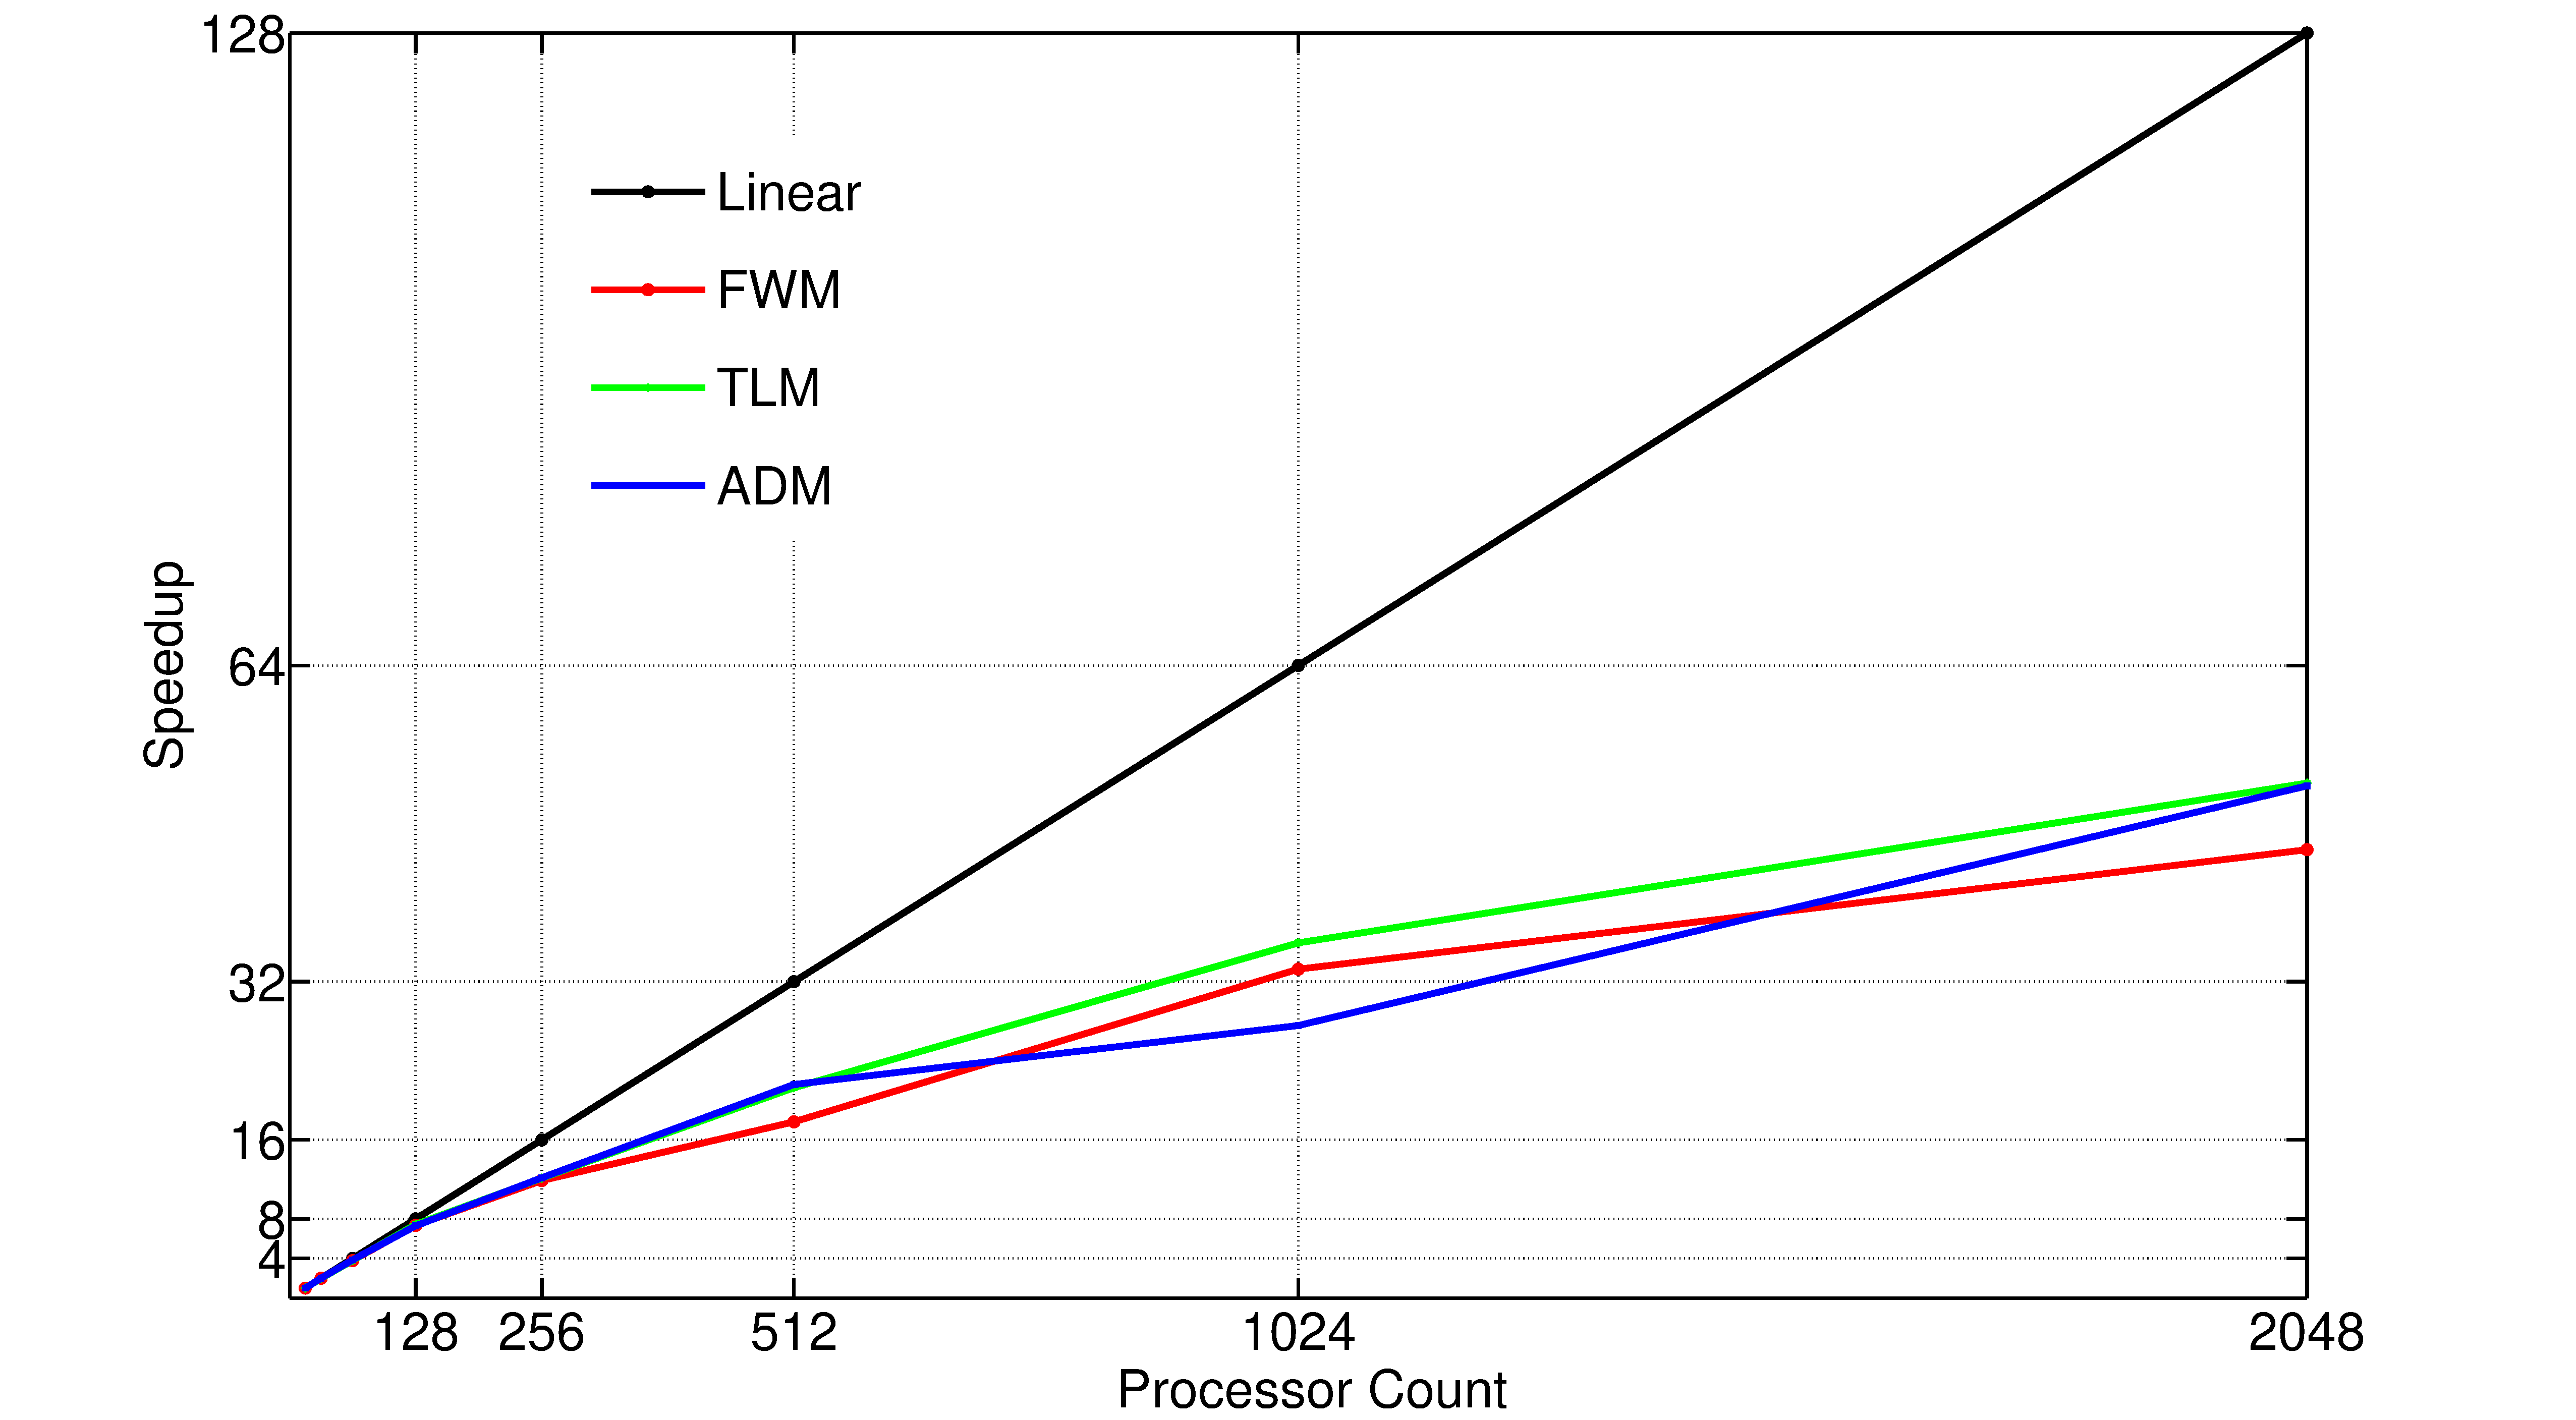
\includegraphics[width=0.8\textwidth]{figures/bluefire_wrfplus_performance.eps}
        }\\ %  ------- End of the first row ----------------------%
%
    \end{center}
    \caption{%
        Parallel performance for one-time-step integration on Bluefire
     }%
   \label{fig:bluefire}
\end{figure}

\begin{figure}[t]
     \begin{center}
%
        \subfigure[Wallclock time for one-time-step integration]{%
            \label{fig:lx_a}
            \includegraphics[width=0.7\textwidth]{lynxtime.pdf}
        }%
        \\
        \subfigure[Parallel speedup]{%
           \label{fig:lx_b}
           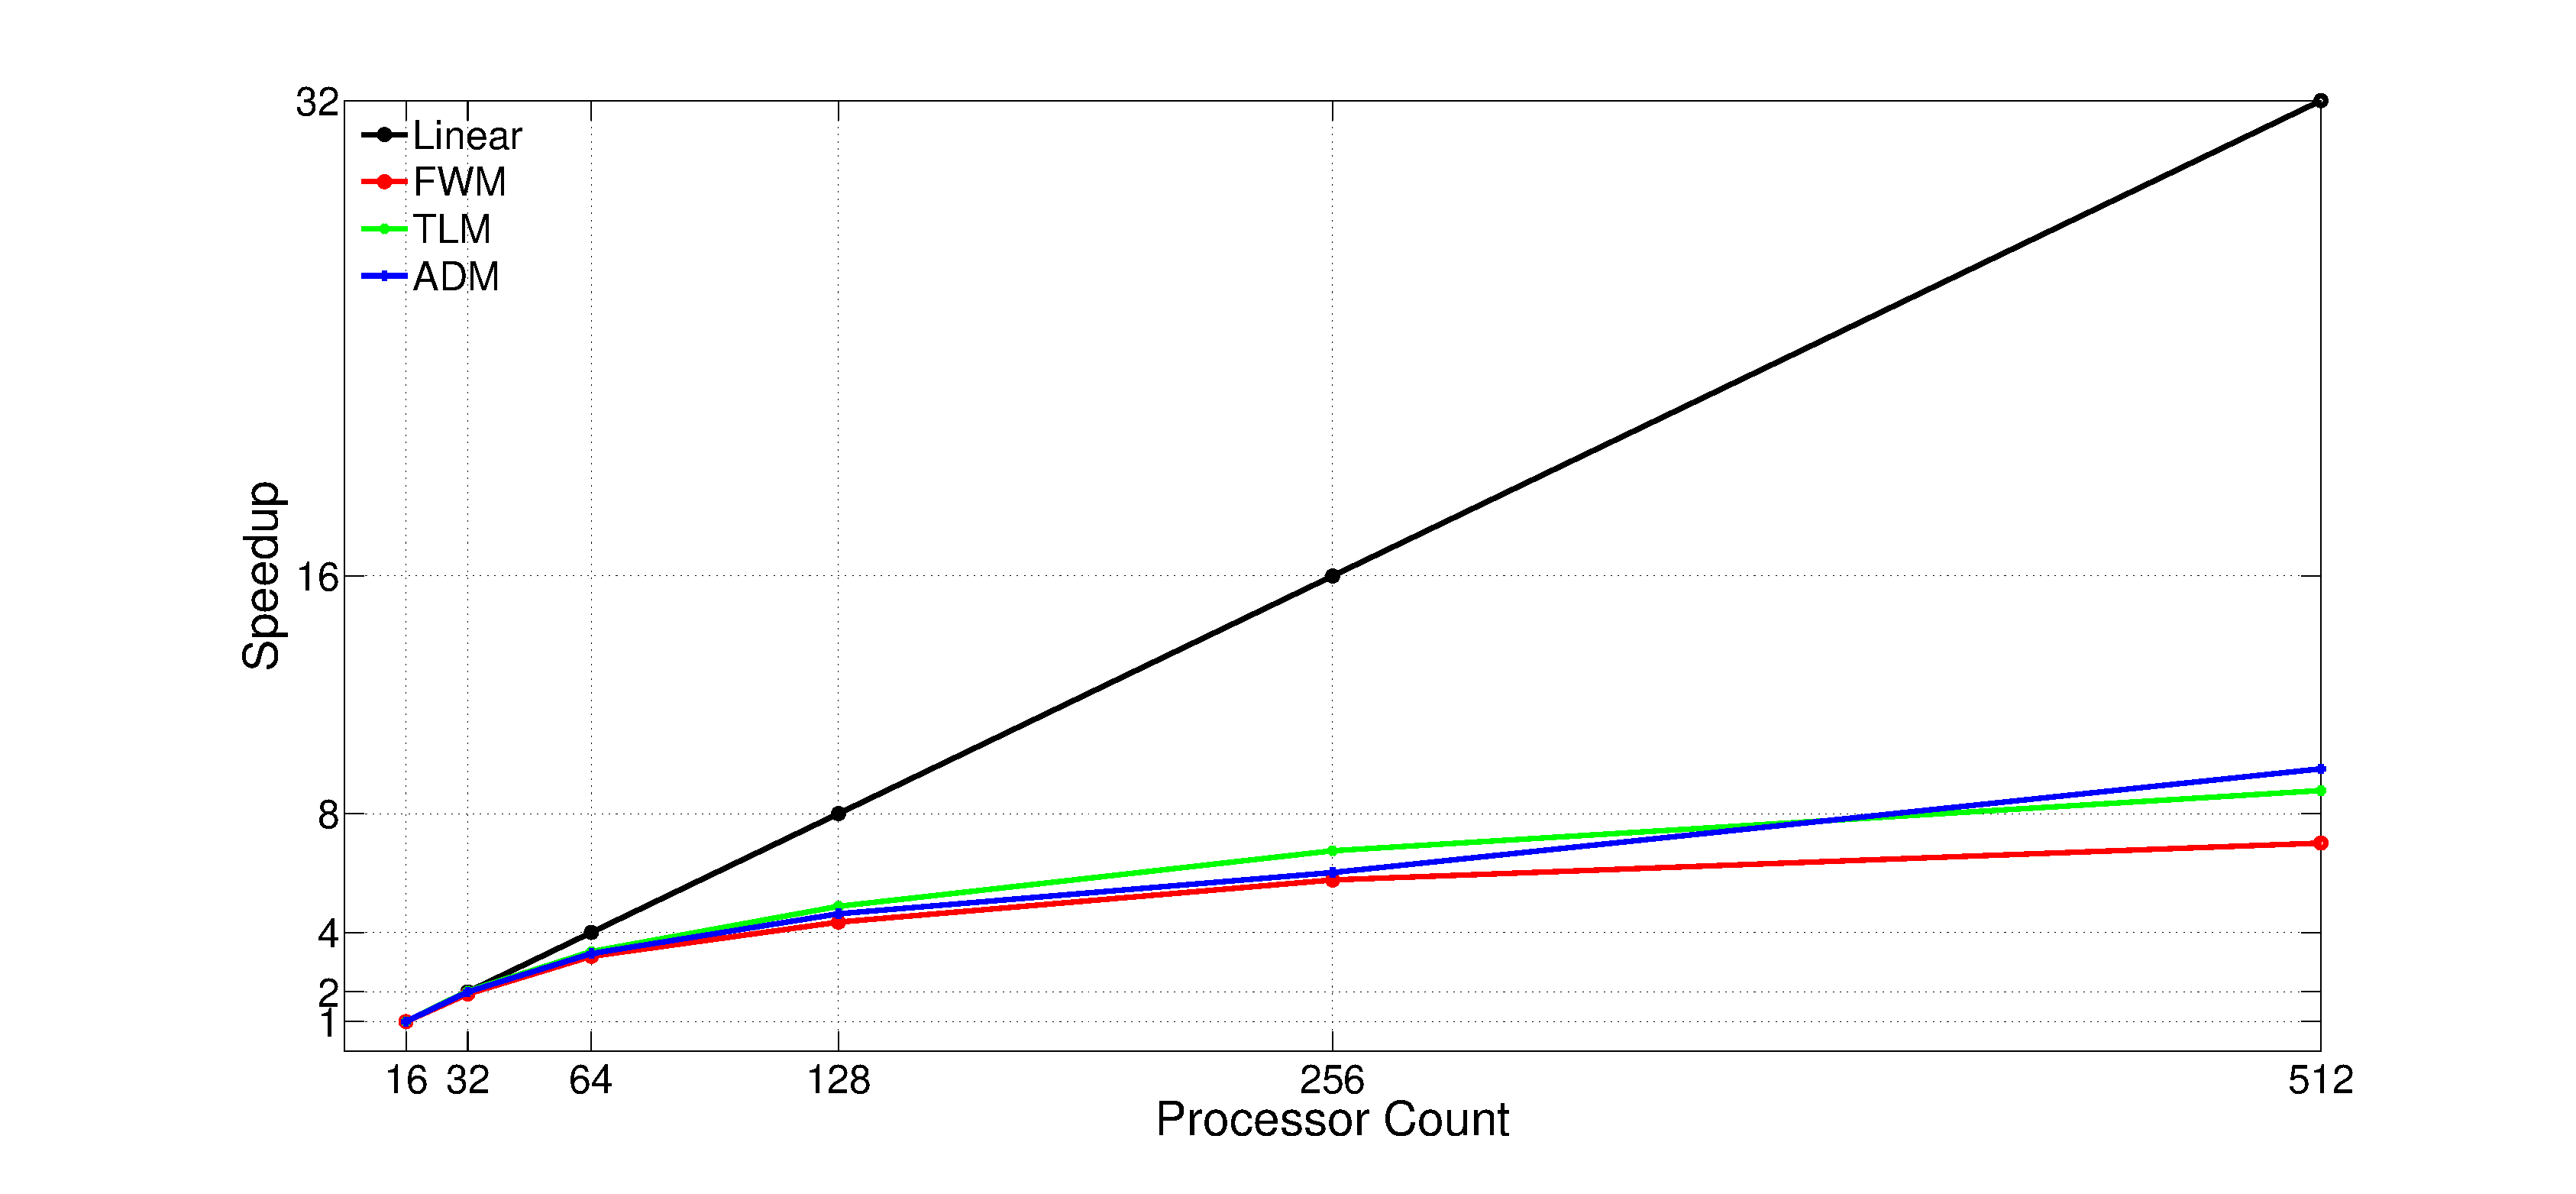
\includegraphics[width=0.8\textwidth]{figures/lynx_wrfplus_performance.eps}
        }\\ %  ------- End of the first row ----------------------%
%
    \end{center}
    \caption{%
        Parallel performance for one-time-step integration on Lynx
     }%
   \label{fig:lynx}
\end{figure}

\begin{figure}[t]
     \begin{center}
%
        \subfigure{%
            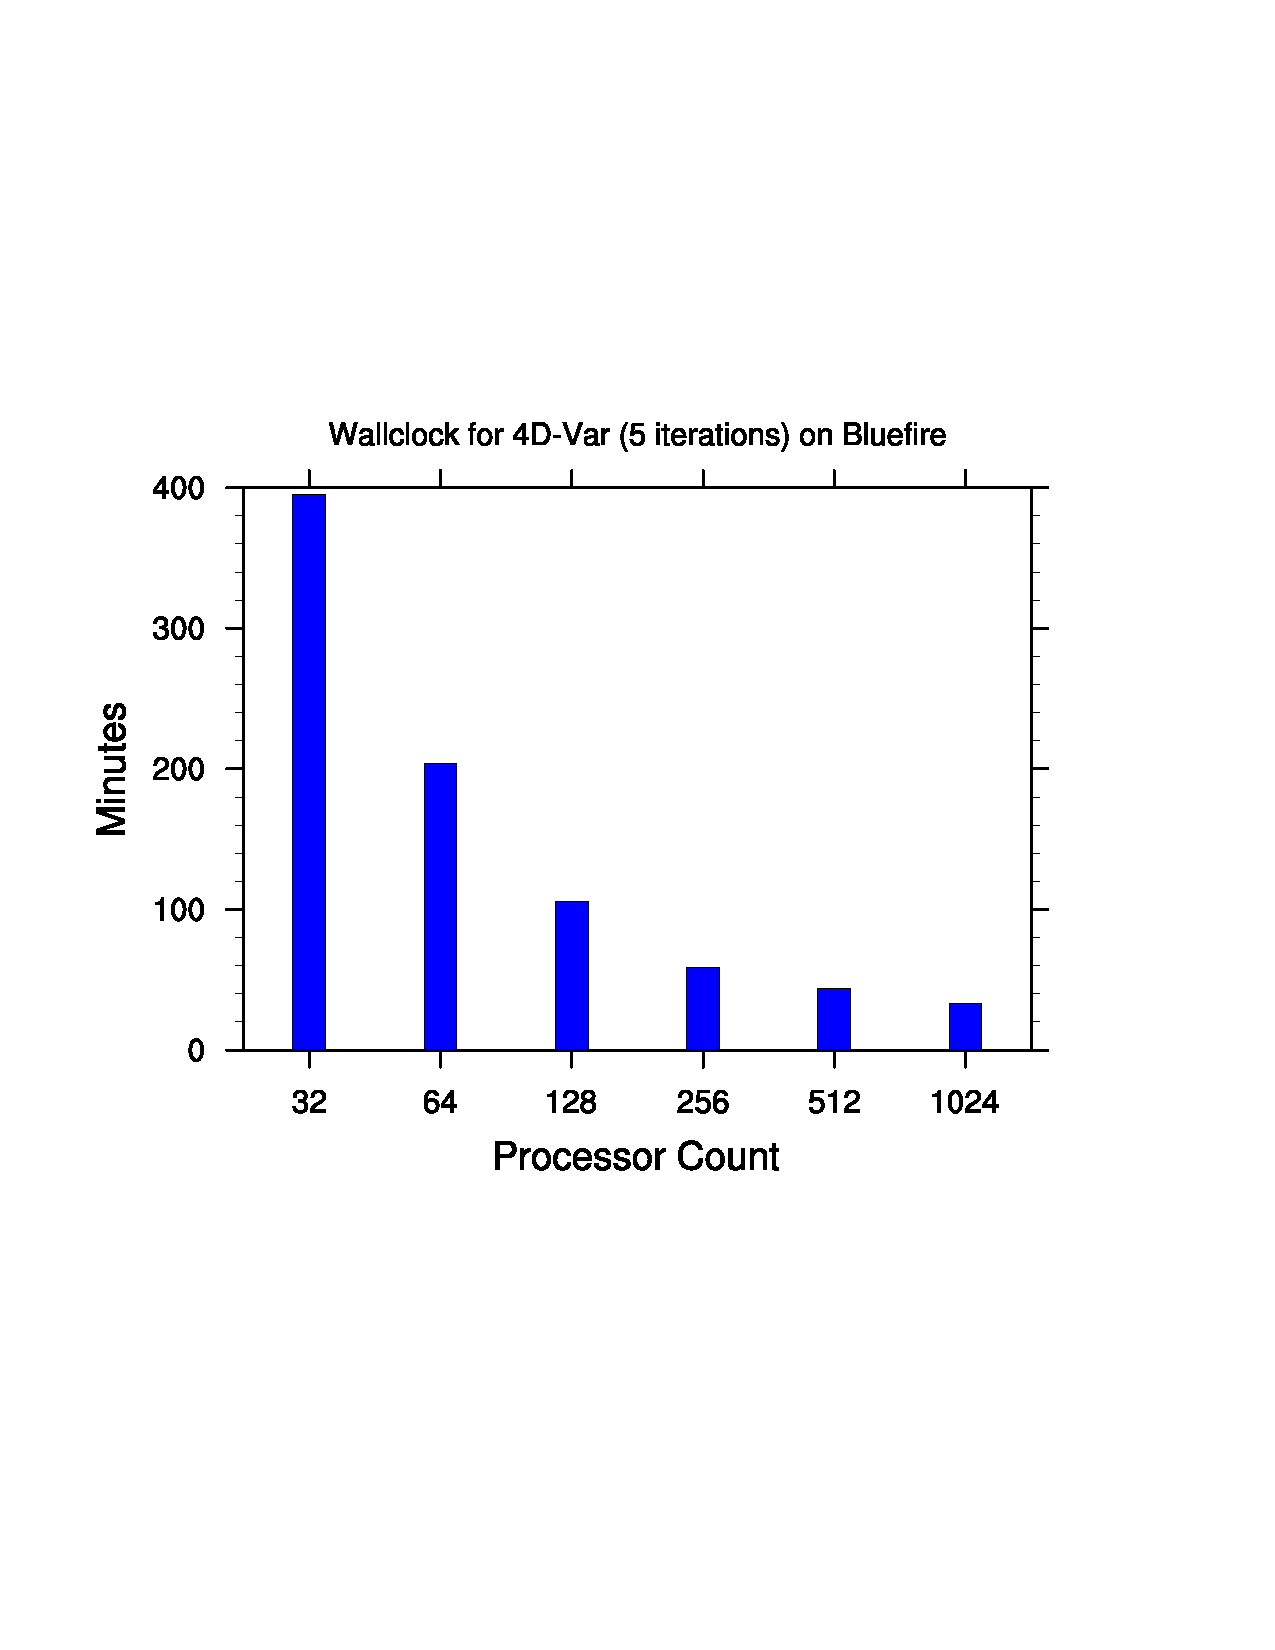
\includegraphics[width=0.7\textwidth]{4dvartime.pdf}
        }%
%
    \end{center}
    \caption{%
        Parallel performance for 4D-Var with 5 iterations on Bluefire
     }%
   \label{fig:4dvar}
\end{figure}


\subsection{Tables}
%%%%%%%%%%%%%%%%%%%%%%%%%%%%%%%%%%%%%%%%%%%%%%%%%%%%%%%%%%%%%%%%%%%%%
% TABLES
%%%%%%%%%%%%%%%%%%%%%%%%%%%%%%%%%%%%%%%%%%%%%%%%%%%%%%%%%%%%%%%%%%%%%
\begin{table}[t]
\caption{Ratio of norms between the tangent linear forecasts and the differences of the two nonlinear model forecasts at 24 h. The norm is defined as the summation of the squares of all variables (perturbations of tangent linear model and difference of two nonlinear models) over the whole domain at 24 h. Here $\lambda$ is the perturbation scaling factors of the initial perturbation.}\label{tlcheck}
\begin{center}
\begin{tabular}{cccccrcrc}
\hline\hline
$\lambda$ & $Ratio$ \\
\hline
.1000E+0 & 0.10114281198481E+01 \\
.1000E-01  & 0.10008545240448E+01 \\
.1000E-02  &  0.10000832484054E+01 \\
.1000E-03  &  0.10000095806229E+01 \\
.1000E-04  &  0.10000007503957E+01 \\
.1000E-05  &  0.10000001743469E+01 \\
.1000E-06  &  0.10000000344215E+01 \\
.1000E-07  &  0.99999998551913E+00 \\
.1000E-08  &  0.10000001453468E+01 \\
.1000E-09  &  0.10000007302081E+01 \\
.1000E-10  &  0.10000775631370E+01 \\
\hline
\end{tabular}
\end{center}
\end{table}


%\begin{table}[t]
%\caption{Parallel performance for one time step integration on Bluefire: ${Wallclock}/{Speedup}$. $Linear$: Linear speedup; $FWM$: Forward model; $TLM$: Tangent linear model; $ADM$: Adjoint model.}\label{bluefire}
%\begin{center}
%\begin{tabular}{cccccrcrc}
%\hline\hline
%$Processors$ & $Linear$ & $FWM$ & $TLM$ & $ADM$ \\
%\hline
%16 & 1 & 4.99s/1.0 & 10.42s/1.0 & 25.91s/1.0 \\
%32 & 2 & 2.49s/2.0 & 5.28s/1.97 & 12.93s/2.0 \\
%64 & 4 & 1.32s/3.78 & 2.74s/3.80 & 6.73s/3.85 \\
%128 & 8 & 0.68s/7.34 & 1.40s/7.44 & 3.55s/7.30 \\
%256 & 16 & 0.42s/11.88 & 0.86s/12.12 & 2.13s/12.16 \\
%512 & 32 & 0.28s/17.82 & 0.49s/21.27 & 1.20s/21.60 \\
%1024 & 64 & 0.15s/33.27 & 0.29s/35.93 & 0.94s/27.56 \\
%2048 & 128 & 0.11s/45.36 & 0.20s/52.10 & 0.50s/51.82 \\
%\hline
%\end{tabular}
%\end{center}
%\end{table}

%
%\begin{table}[t]
%\caption{Parallel performance for one time step integration on Lynx: ${Wallclock}/{Speedup}$. $Linear$: Linear speedup; $FWM$: Forward model; $TLM$: Tangent linear model; $ADM$: Adjoint model..}\label{lynx}
%\begin{center}
%\begin{tabular}{cccccrcrc}
%\hline\hline
%$Processors$ & $Linear$ & $FWM$ & $TLM$ & $ADM$ \\
%\hline
%16 & 1 & 6.52s/1.0 & 15.80s/1.0 & 33.20s/1.0 \\
%32 & 2  & 3.37s/1.93  & 7.78s/2.03 & 16.63s/2.0 \\
%64 & 4 & 2.04s/3.20 & 4.70s/3.36 & 10.12s/3.29 \\
%128 & 8 & 1.50s/4.35 & 3.24s/4.88 & 7.20s/4.63 \\
%256 & 16 & 1.13s/5.77 & 2.43s/6.75 & 5.53s/6.02 \\
%512 & 32 & 0.93s/7.01 & 1.80s/8.78 & 3.50s/9.51 \\
%\hline
%\end{tabular}
%\end{center}
%\end{table}

%%%%%%%%%%%%%%%%%%%%%%%%%%%%%%%%%%%%%%%%%%%%%%%%%%%%%%%%%%%%%%%%%%%%%
% ACKNOWLEDGMENTS
%%%%%%%%%%%%%%%%%%%%%%%%%%%%%%%%%%%%%%%%%%%%%%%%%%%%%%%%%%%%%%%%%%%%%

\begin{acknowledgment}
The National Center for Atmospheric Research is sponsored by the National
Science Foundation.  This work is supported by the Air Force Weather Agency. The WRFPLUS system has benefitted greatly from close collaboration with Dr. Qiang Chen and his ADG tools. We thank Dong-Kyou Lee and Gyu-Ho Lim of Seoul National University for their comments on the manuscript and generous support through KUWCC. We thank Fuqing Zhang and Jon Poterjoy of Penn State University for their valuable suggestions and comments on the manuscript.
\end{acknowledgment}


%%%%%%%%%%%%%%%%%%%%%%%%%%%%%%%%%%%%%%%%%%%%%%%%%%%%%%%%%%%%%%%%%%%%%
% REFERENCES
%%%%%%%%%%%%%%%%%%%%%%%%%%%%%%%%%%%%%%%%%%%%%%%%%%%%%%%%%%%%%%%%%%%%%
% Create a bibliography directory and place your .bib file there.
\ifthenelse{\boolean{dc}}
{}
{\clearpage}
\bibliographystyle{ametsoc}
%\bibliography{../bibliography/references}
\bibliography{references}
\end{document}
%%%%%%%%%%%%%%%%%%%%%%%%%%%%%%%%%%%%%%%%%%%%%%%%%%%%%%%%%%%%%%%%%%%%%
% END OF TEMPLATE
%%%%%%%%%%%%%%%%%%%%%%%%%%%%%%%%%%%%%%%%%%%%%%%%%%%%%%%%%%%%%%%%%%%%%
